% Sequential heatmap with exact values; one common 0--1 colour scale.
\begingroup
\definecolor{classFOne}{RGB}{55,126,184}
\newcommand{\fOneCell}[2]{\cellcolor{classFOne!#1!white}\color{black}#2}
\small
\renewcommand{\arraystretch}{1.5}
\setlength{\tabcolsep}{7pt}
\begin{tabular}{lrrrr}
 & \textbf{Anger} & \textbf{Happiness} & \textbf{Neutral} & \textbf{Sadness} \\
Utterance-only text & \fOneCell{71.52}{0.7152} & \fOneCell{71.8}{0.7180} & \fOneCell{60.67}{0.6067} & \fOneCell{62.05}{0.6205} \\
Three-turn context & \fOneCell{73.49}{0.7349} & \fOneCell{80.62}{0.8062} & \fOneCell{64.04}{0.6404} & \fOneCell{75.12}{0.7512} \\
Audio only & \fOneCell{71.42}{0.7142} & \fOneCell{57.82}{0.5782} & \fOneCell{57.57}{0.5757} & \fOneCell{67.15}{0.6715} \\
Equal-weight fusion & \fOneCell{82.77}{0.8277} & \fOneCell{81.63}{0.8163} & \fOneCell{70.14}{0.7014} & \fOneCell{80.8}{0.8080} \\
Validation-fitted fusion & \fOneCell{79.51}{0.7951} & \fOneCell{82.21}{0.8221} & \fOneCell{68.97}{0.6897} & \fOneCell{79.61}{0.7961} \\
\end{tabular}
\par\smallskip
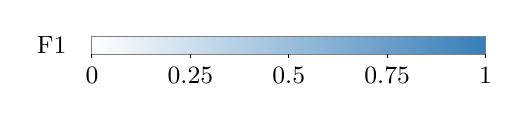
\begin{tikzpicture}[x=5cm,y=0.23cm,font=\small]
  \shade[left color=white,right color=classFOne] (0,0) rectangle (1,1);
  \draw[gray] (0,0) rectangle (1,1);
  \foreach \value in {0,0.25,0.5,0.75,1} {
    \draw (\value,0) -- (\value,-0.2);
    \node[anchor=north] at (\value,-0.2) {\value};
  }
  \node[anchor=east] at (-0.04,0.5) {F1};
\end{tikzpicture}
\endgroup
